\subsection{pbdMPI Example: Random Forest Prediction}
\makesubcontentsslidessec


\begin{frame}[fragile]{Letter Recognition Data}
  \begin{exampleblock}{Example \countex : Letter Recognition data from
      package \pkg{mlbench} (20,000 $\times$ 17)}\pause
    \vspace{-1em}
    \begin{minipage}{0.3\textwidth}
      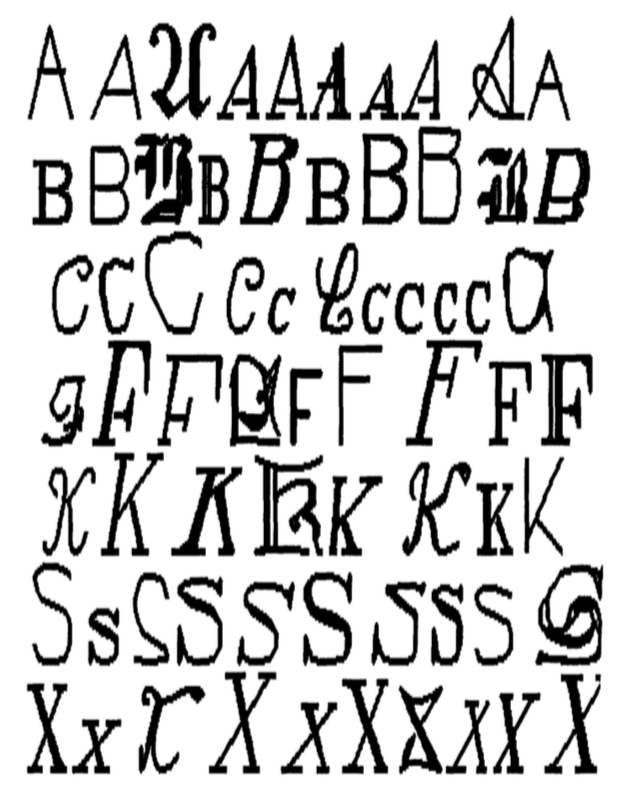
\includegraphics[width=0.95\textwidth]{../common/pics/apps/ML_FreySlate1991}
    \end{minipage}
    \begin{minipage}{0.69\textwidth}\tiny
      \begin{lstlisting}
[,1]	lettr	capital letter
[,2]	x.box	horizontal position of box
[,3]	y.box	vertical position of box
[,4]	width	width of box
[,5]	high	height of box
[,6]	onpix	total number of on pixels
[,7]	x.bar	mean x of on pixels in box
[,8]	y.bar	mean y of on pixels in box
[,9]	x2bar	mean x variance
[,10]	y2bar	mean y variance
[,11]	xybar	mean x y correlation
[,12]	x2ybr	mean of x^2 y
[,13]	xy2br	mean of x y^2
[,14]	x.ege	mean edge count left to right
[,15]	xegvy	correlation of x.ege with y
[,16]	y.ege	mean edge count bottom to top
[,17]	yegvx	correlation of y.ege with x
      \end{lstlisting}
    \end{minipage} \\
    {\tiny P. W. Frey and D. J. Slate (Machine Learning Vol 6/2 March 91):
    "Letter Recognition Using Holland-style Adaptive Classifiers".}
  \end{exampleblock}
\end{frame}


\begin{frame}
  \begin{exampleblock}{Example \showex : Random Forest Algorithm}\pause
    \begin{enumerate}
     \item Build simple regression trees from random subsets of
       columns
     \item Use model averaging for prediction
     \item Package \pkg{randomForest} has a \code{combine()} function
       that enables the following parallel approach:
       \begin{enumerate}
       \item Everyone gets the same training data
       \item Split regression tree building among processors
         (\pkg{randomForest})
       \item Use \code{allgather} to bring built predictors to all
       \item Everyone \code{combine} predictors
       \item Split prediction work by blocks of rows
       \item Use \code{allreduce} to assess prediction
       \end{enumerate}
     \item Steps (3) and (4) can be improved with a custom
       reduce/combine to take advantage of MPI vendor optimizations
    \end{enumerate}
  \end{exampleblock}
\end{frame}


\begin{frame}[fragile]
  \begin{exampleblock}{Example \showex :  Random Forest Code \\
      (Split learning by blocks of trees. Split prediction by blocks
      of rows.)}\pause
    \begin{lstlisting}[title=Serial Code 4\_rf\_s.r]
library(randomForest)
library(mlbench)
data(LetterRecognition) # 26 Capital Letters Data 20,000 x 17
set.seed(seed=123)
n <- nrow(LetterRecognition)
n_test <- floor(0.2*n)
i_test <- sample.int(n, n_test) # Use 1/5 of the data to test
train <- LetterRecognition[-i_test, ]
test <- LetterRecognition[i_test, ]

## train random forest
rf.all <- randomForest(lettr ~ ., train, ntree=500, norm.votes=FALSE)

## predict test data
pred <- predict(rf.all, test)
correct <- sum(pred == test$lettr)
cat("Proportion Correct:", correct/(n_test), "\n")
    \end{lstlisting} %$
  \end{exampleblock}
\end{frame}


\begin{frame}[fragile]
  \begin{exampleblock}{Example \showex :  Random Forest Code \\
      (Split learning by blocks of trees. Split prediction by blocks
      of rows.)}\pause
    \begin{lstlisting}[title=Parallel Code 4\_rf\_p.r,escapeinside={(*@}{@*)}]
library(randomForest)
library(mlbench)
data(LetterRecognition)
(*@\textcolor{red}{comm.}@*)set.seed(seed=123(*@\textcolor{red}{, diff=FALSE}@*)) # same training data
n <- nrow(LetterRecognition)
n_test <- floor(0.2*n)
i_test <- sample.int(n, n_test) # Use 1/5 of the data to test
train <- LetterRecognition[-i_test, ]
test <- LetterRecognition[i_test, ](*@\textcolor{red}{[get.jid(n\_test), ]}@*)

(*@\textcolor{red}{comm.set.seed(seed=1e6*runif(1), diff=TRUE)}@*)
my.rf <- randomForest(lettr ~ ., train, ntree=500(*@\textcolor{red}{\%/\%comm.size()}@*), norm.votes=FALSE)
(*@\textcolor{red}{rf.all <- do.call(combine, allgather(my.rf))}@*)

pred <- predict(rf.all, test)
correct <- (*@\textcolor{red}{allreduce(}@*)sum(pred == test$lettr)(*@\textcolor{red}{)}@*)
(*@\textcolor{red}{comm.}@*)cat("Proportion Correct:", correct/(n_test), "\n")
    \end{lstlisting} %$
  \end{exampleblock}
\end{frame}

\begin{frame}[fragile]
\begin{block}{Runs serial or on any number of cores}
\vspace{-2ex}
\begin{lstlisting}[escapeinside={(*@}{@*)}]
[beacon-login2 stats]$ time (*@\textcolor{red}{Rscript 4\_rf\_s.r}@*)
Proportion Correct: 0.96725
real	(*@\textcolor{red}{0m49.028s}@*)   user	0m48.626s    sys	0m0.335s
[beacon-login2 stats]$ time (*@\textcolor{red}{Rscript 4\_rf\_p.r}@*)
Proportion Correct: 0.96425
real	(*@\textcolor{red}{0m52.634s}@*)   user	0m51.914s    sys	0m0.598s
[beacon-login2 stats]$ time (*@\textcolor{red}{mpirun -np 2 Rscript 4\_rf\_p.r}@*)
Proportion Correct: 0.96425
real	(*@\textcolor{red}{0m28.349s}@*)   user	0m54.570s    sys	0m1.070s
[beacon-login2 stats]$ time (*@\textcolor{red}{mpirun -np 4 Rscript 4\_rf\_p.r}@*)
Proportion Correct: 0.963
real	(*@\textcolor{red}{0m16.380s}@*)   user	1m1.559s     sys	0m1.664s
[beacon-login2 stats]$ time (*@\textcolor{red}{mpirun -np 8 Rscript 4\_rf\_p.r}@*)
Proportion Correct: 0.963
real	(*@\textcolor{red}{0m11.010s}@*)   user	1m19.301s    sys	0m3.421s
[beacon-login2 stats]$ time (*@\textcolor{red}{mpirun -np 16 Rscript 4\_rf\_p.r}@*)
Proportion Correct: 0.9635
real	(*@\textcolor{red}{0m10.655s}@*)   user	2m32.508s    sys	0m6.624s
[beacon-login2 stats]$ time (*@\textcolor{red}{mpirun -np 32 Rscript 4\_rf\_p.r}@*)
Proportion Correct: 0.96325
real	(*@\textcolor{red}{0m21.692s}@*)   user	4m44.114s    sys	0m20.179s
\end{lstlisting}
\end{block}
\end{frame}